\newpage
\section{Windows Presentation Foundation (WPF)}

\subsection{Counter Application}

\begin{figure}[htbp]
	\centering
	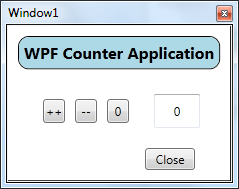
\includegraphics[width=6cm]{images/WPF_Counter.png}
\end{figure}

MainWindows.xaml:
\begin{lstlisting}[style=Csharp]
<Window x:Class="GUI.MainWindow"
        xmlns="http://schemas.microsoft.com/winfx/2006/xaml/presentation"
        xmlns:x="http://schemas.microsoft.com/winfx/2006/xaml"
        Title="Window1" WindowStyle="ToolWindow" mc:Ignorable="d" xmlns:d="http://schemas.microsoft.com/expression/blend/2008" xmlns:mc="http://schemas.openxmlformats.org/markup-compatibility/2006" d:DesignHeight="200" d:DesignWidth="300" SizeToContent="WidthAndHeight">
    <StackPanel Margin="10">
        <Border BorderBrush="Black" Background="LightBlue" BorderThickness="1" CornerRadius="10">
            <Label FontWeight="Bold" FontSize="16" HorizontalAlignment="Center" >WPF Counter Application</Label>
        </Border>
        <DockPanel LastChildFill="True" Margin="10 15 10 10" >
            <StackPanel Margin="10" Orientation="Horizontal">
                <Button Margin="5 5 5 5" Width="22" Height="24" Click="pp_Click">++</Button>
                <Button Margin="5 5 5 5" Width="22" Height="24" Click="mm_Click">--</Button>
                <Button Margin="5 5 5 5" Width="22" Height="24" Click="res_Click">0</Button>
            </StackPanel>
            <TextBox Margin="10" TextAlignment="Center" VerticalContentAlignment="Center" x:Name="mCountValue" IsReadOnly="True" Text="{Binding Path=Count, Mode=OneWay}"></TextBox>
        </DockPanel>
        <Button Width="50" HorizontalAlignment="Right" Margin="0 0 25 0" Click="close_Click" >Close</Button>
        <!-- Counter GUI Controls -->

    </StackPanel>
</Window>
\end{lstlisting}

\newpage
Corresponding MainWindow.xaml.cs
\begin{lstlisting}[style=Csharp]
namespace GUI
{
    public partial class MainWindow : Window
    {
        private ICounter count1;

        public MainWindow()
        {
            InitializeComponent();
            count1 = new CounterImpl();
            //count1.CountChanged += Counter_CountChanged;
            DataContext = count1;
        }

        public MainWindow(ICounter myCounter)
        {
            InitializeComponent();
            count1 = myCounter;
            DataContext = count1;
        }

        private void pp_Click(object sender, RoutedEventArgs e)
        {
            count1.Increment();

        }

        private void mm_Click(object sender, RoutedEventArgs e)
        {
            count1.Decrement();
        }

        private void res_Click(object sender, RoutedEventArgs e)
        {
            count1.Reset();
        }

        private void close_Click(object sender, RoutedEventArgs e)
        {
            Close();
        }

        private void Counter_CountChanged(ICounter sender, CountChangedEventArgs e)
        {
            mCountValue.Text = e.NewValue.ToString();
        }

    }
}
\end{lstlisting}
